
\section{API}

همانطور که اشاره کردم بخش API پروژه از زبان Go و فریمورک Fiber استفاده می‌کند.
این پروژه لایه ورودی ما به بخش های داخلی سیستم می‌باشد.

در عکس زیر نمایی از api های موجود در پروژه مشاهده می‌شود.
این api ها در چند دسته مختلف تقسیم بندی شده اند. sandbox برای ساخت یک پروژه جدید و اجرا آن می‌باشد.
بخش auth برای ثبت نام و ورود کاربر است.
بخش user برای دریافت اطلاعات کاربر وارد شده است.
و health برای بررسی liveness و readiness سیستم در نظر گرفته شده است.
وجود این مسیر باعث می‌شود در سیستم های مدیریت کانتینر مانند kubernetes از آمادگی سرویس اطمینان حاصل کرد.

\begin{figure}[hb]
    \centering
    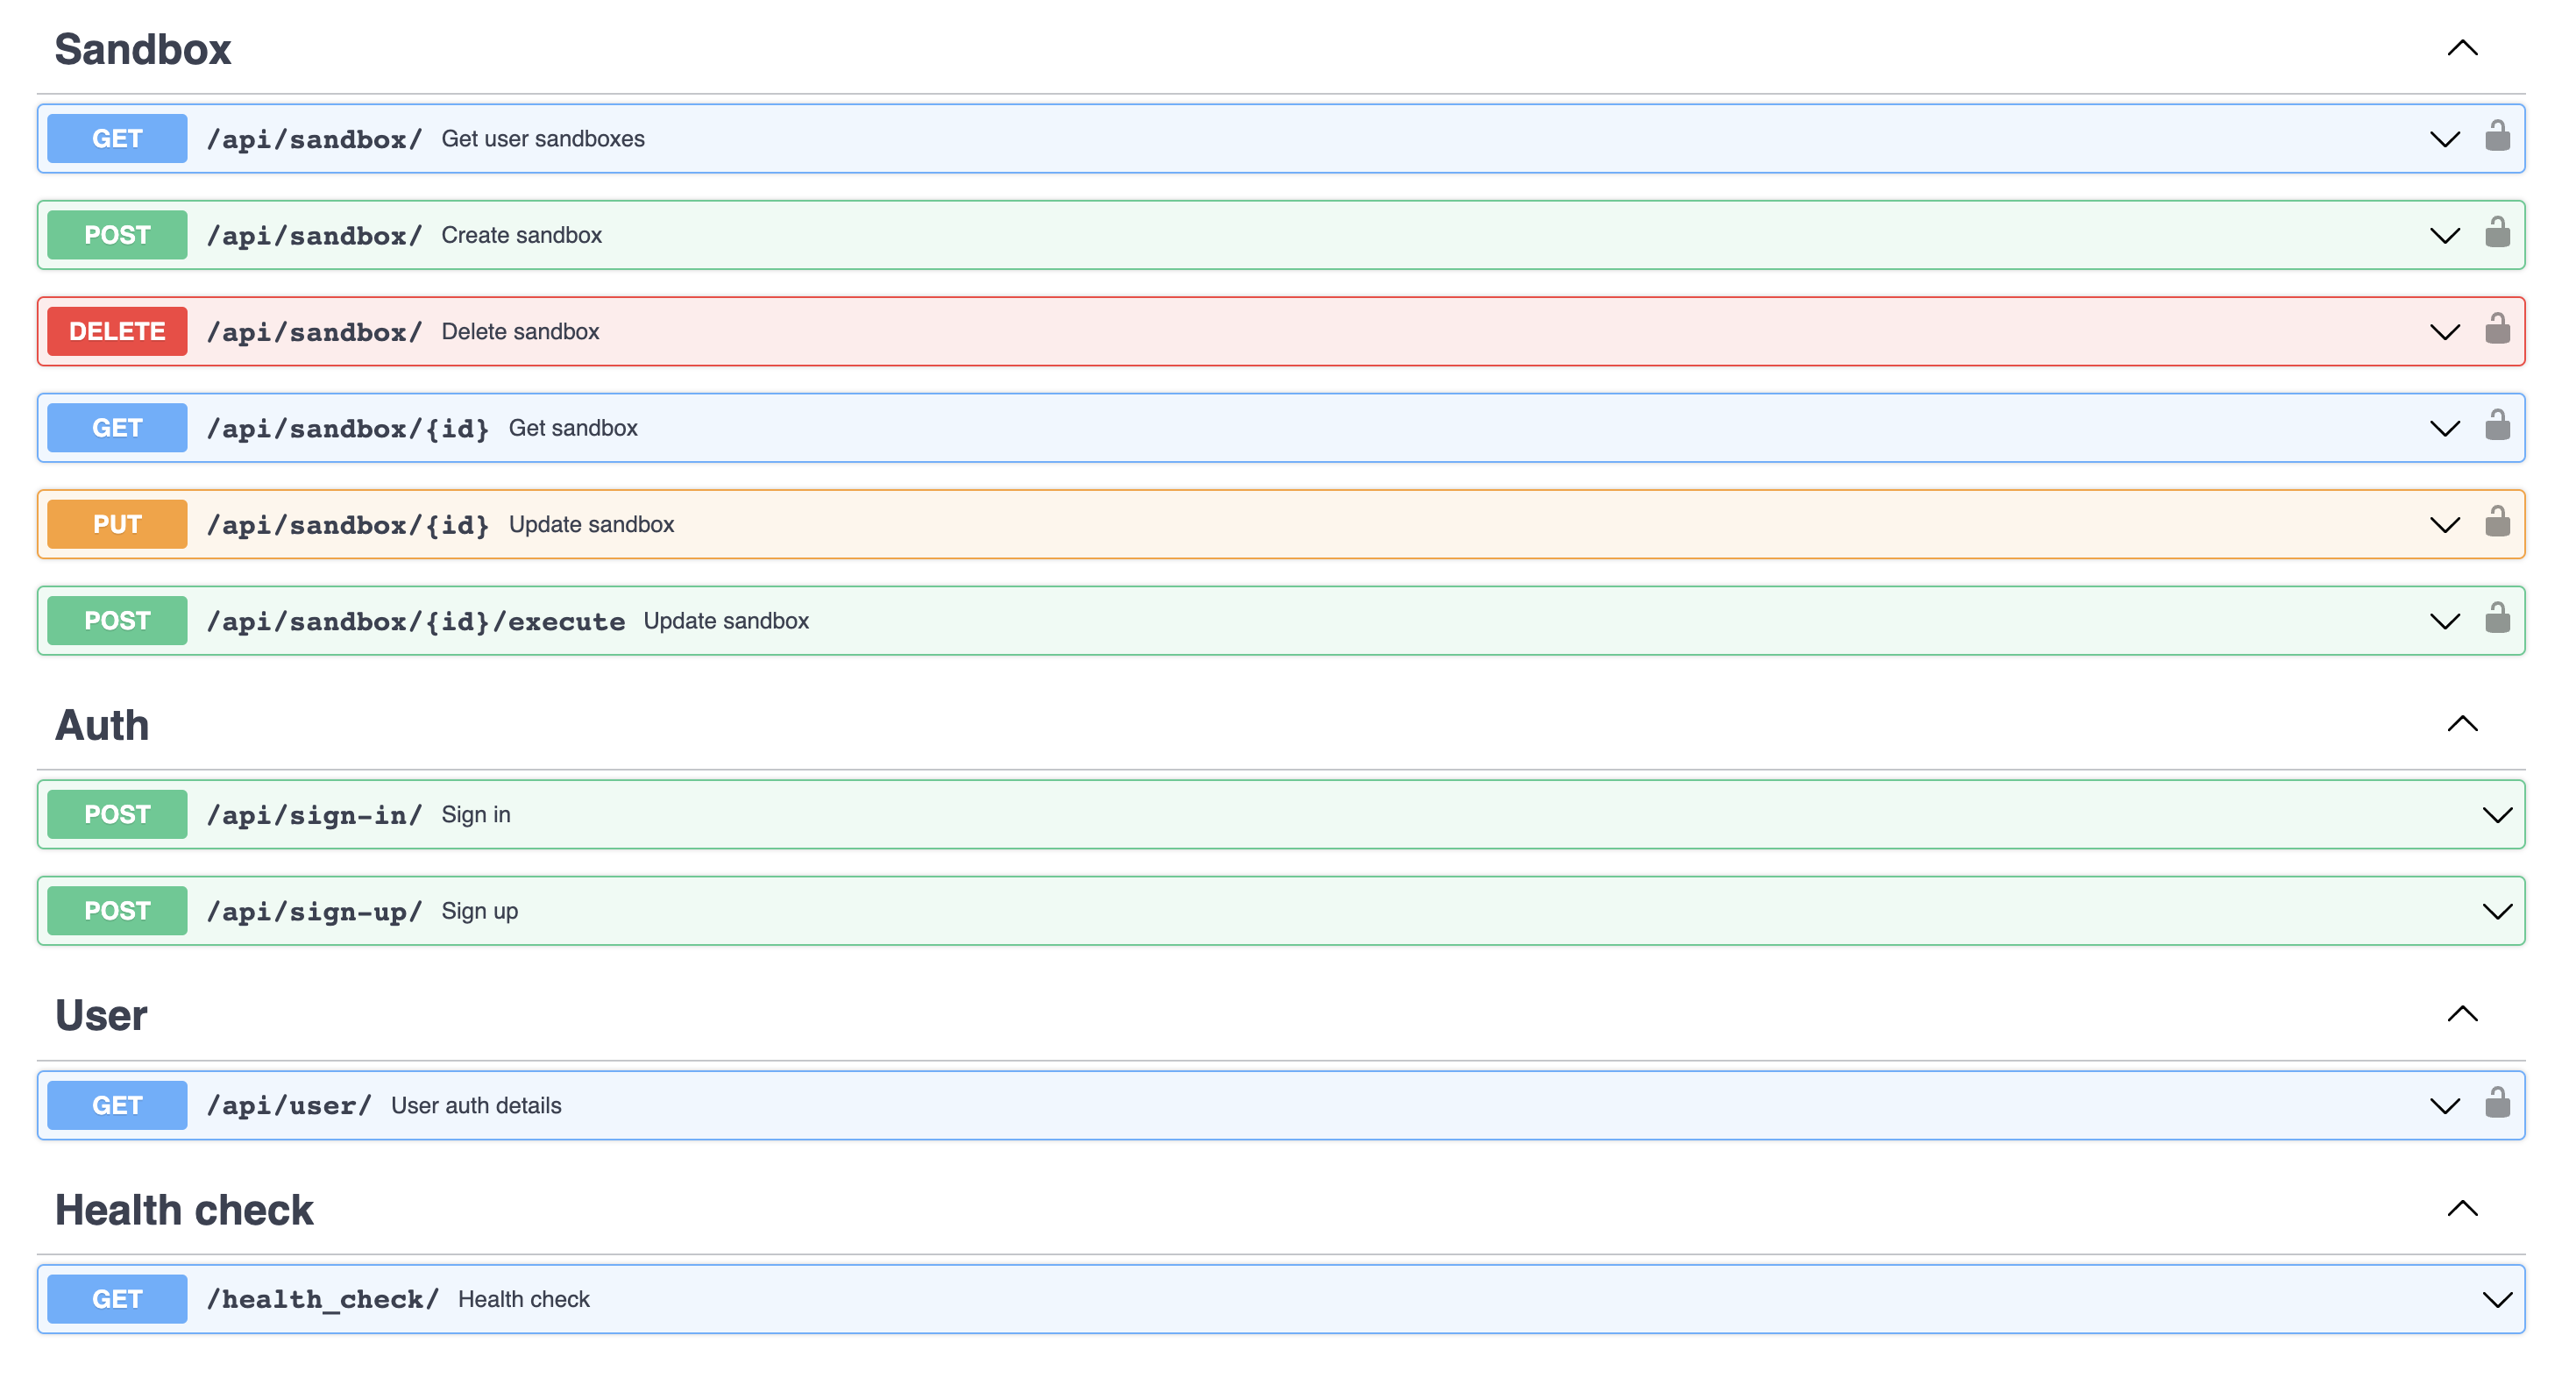
\includegraphics[width=1\textwidth]{./3-Design/swagger.png}
    \caption{لیست API}
    \label{fig:swagger}
\end{figure}
